\titre{Numerical simulations of LZ78 for Markovian sources}
% Veuillez ne pas modifier ce titre SVP.
% En cas de doute, pr�venez votre coordinateur.
% Compilez par: "latex main.tex".


\separation
\bk

% Quelques explications sur le sujet; articulation des parties; une page.



%%%%%%%%%%%%%%%%%%%%%%%%%%%%%%%%%%%%%%%%%%%%%%%%%%%%%%%%%%%%%%%%%%%%%%%%%%%%%%



\medskip

	\centers{\question{Simulation}}

This	 document presents the different graphics I obtained during the following experimental
process :
	
\begin{itemize}

	\item Generating a random Markov chain of size 2 of matrix
 \centers{ $\begin{matrice}
			p_{0 0} & p_{0 1} \\
			p_{1 0} & p_{1 1} \\
		  \end{matrice}$}	 
 \item
 Generating $n_{\text{exp}} \sim 500$ words of length $n $ (or $n_{\text{word}}$), with $n \leq 10^6$
 
 \item Applying LZ78 on each of these words to estimate, for each $n$,
 the number of phrases $M_n$. A simple histogram of these values
 can be seen in figure 1.
 
 \item From this sampling of the random variable $M_n$ and other parameters such as the entropy of the Markov chain, computing
 
 	\begin{itemize}
 		\item the empirical mean ($\mu$) and the empirical variance ($\sigma^2$)
 		\item different theoretical expressions of the mean and variance
 	\end{itemize}
 	
 \item Using these expressions to standardize $M_n$ in different ways, plotting
 
 	\begin{itemize}
 		\item the probability distribution of $M_n$ (standardized)
 			  
 		\item the cumulative distribution function of $M_n$ (standardized)
 	\end{itemize}
 
 \item Finally, comparing the different theoretical expressions for the mean and 
 variance by plotting their differences for a large range of values of $n$, and
 a constant number of experiments $n_{\text{exp}}$.
\end{itemize}
 
 
 This histogram represents the counts of the different 
 values taken by $M_n$ for $n=10^6$. 
 Each tick on the x-axis is a data point.
 
 \centers{
  \begin{minipage}{7cm}
   
    		
        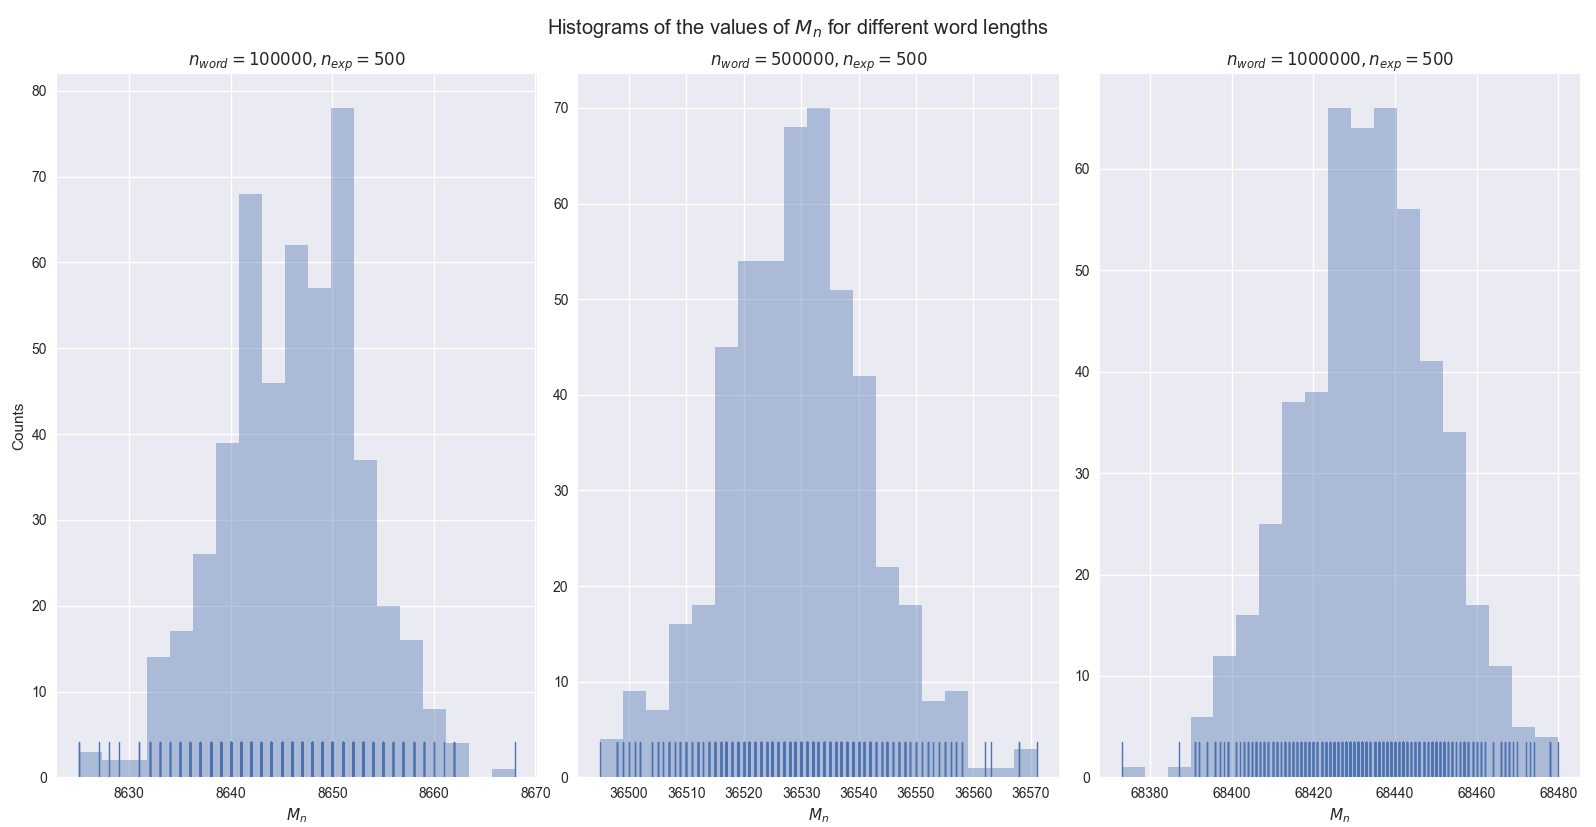
\includegraphics[width = 7cm,
        				    trim = 27cm 0 0 0,
        				    	clip=true]{M_n_raw_10e6_500.png}	
       
    
	\end{minipage}
}

 		\centers{\question{Empirical normalization}}
 Using the empirical mean ($\mu$) and variance ($\sigma^2$) of the dataset to normalize $M_n$,
 this is a plot of the normalized distribution, compared to the normal distribution 
 in red :
 \centers{
  \begin{minipage}{6cm}
        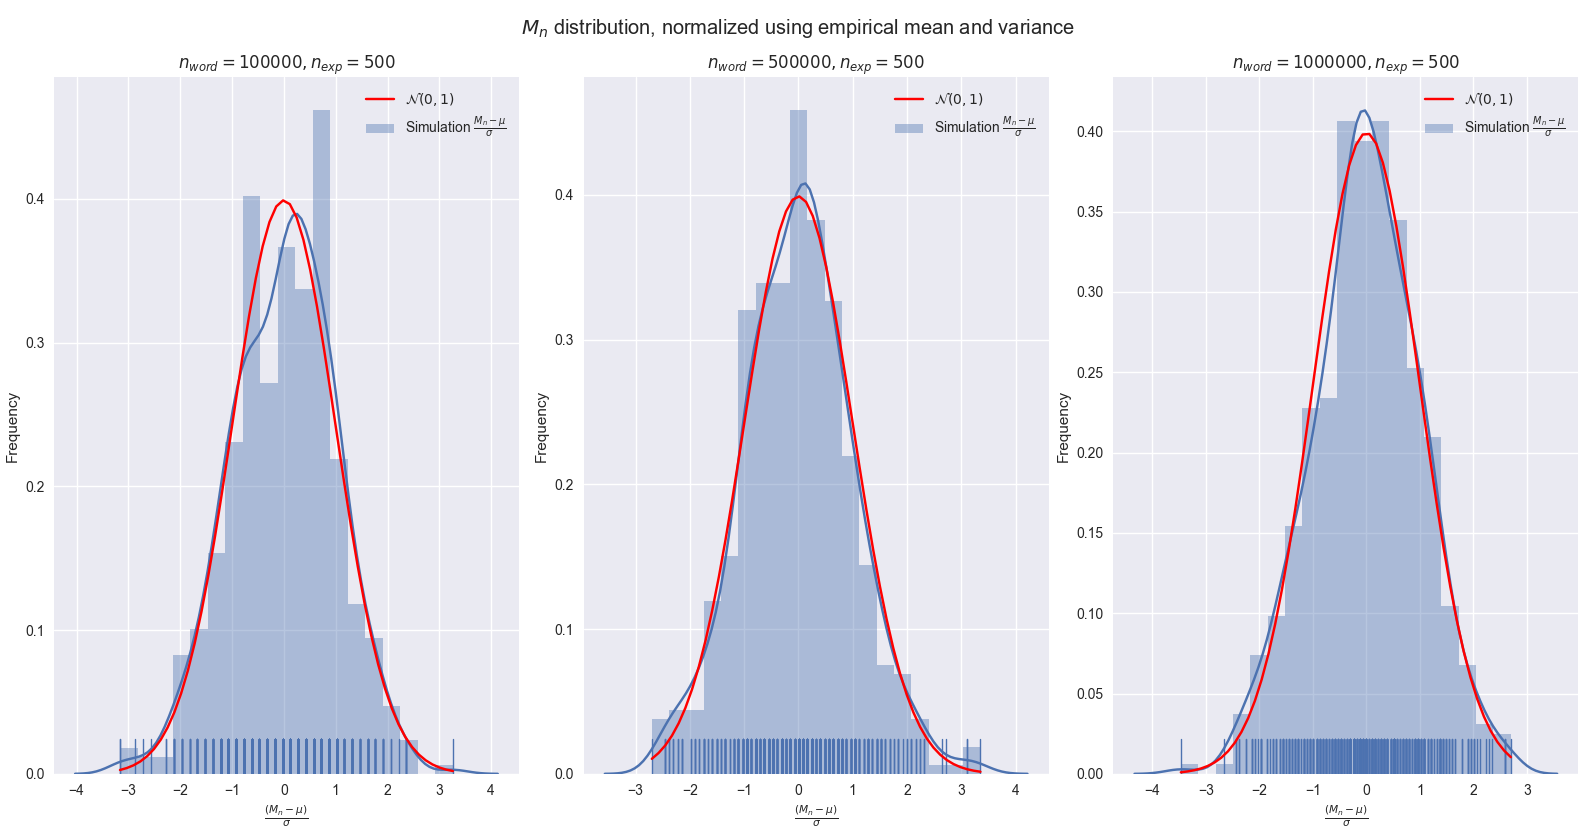
\includegraphics[width = 6cm,
        				    trim = 26.7cm 0 0 30,
        				    	clip=true]{empirical_normalization_10e6_500.png}	
	\end{minipage} 
}
	\noindent
	 and its cumulative distribution function in green, compared to the normal one in red:
 	\centers{
 	 \begin{minipage}{7cm}
        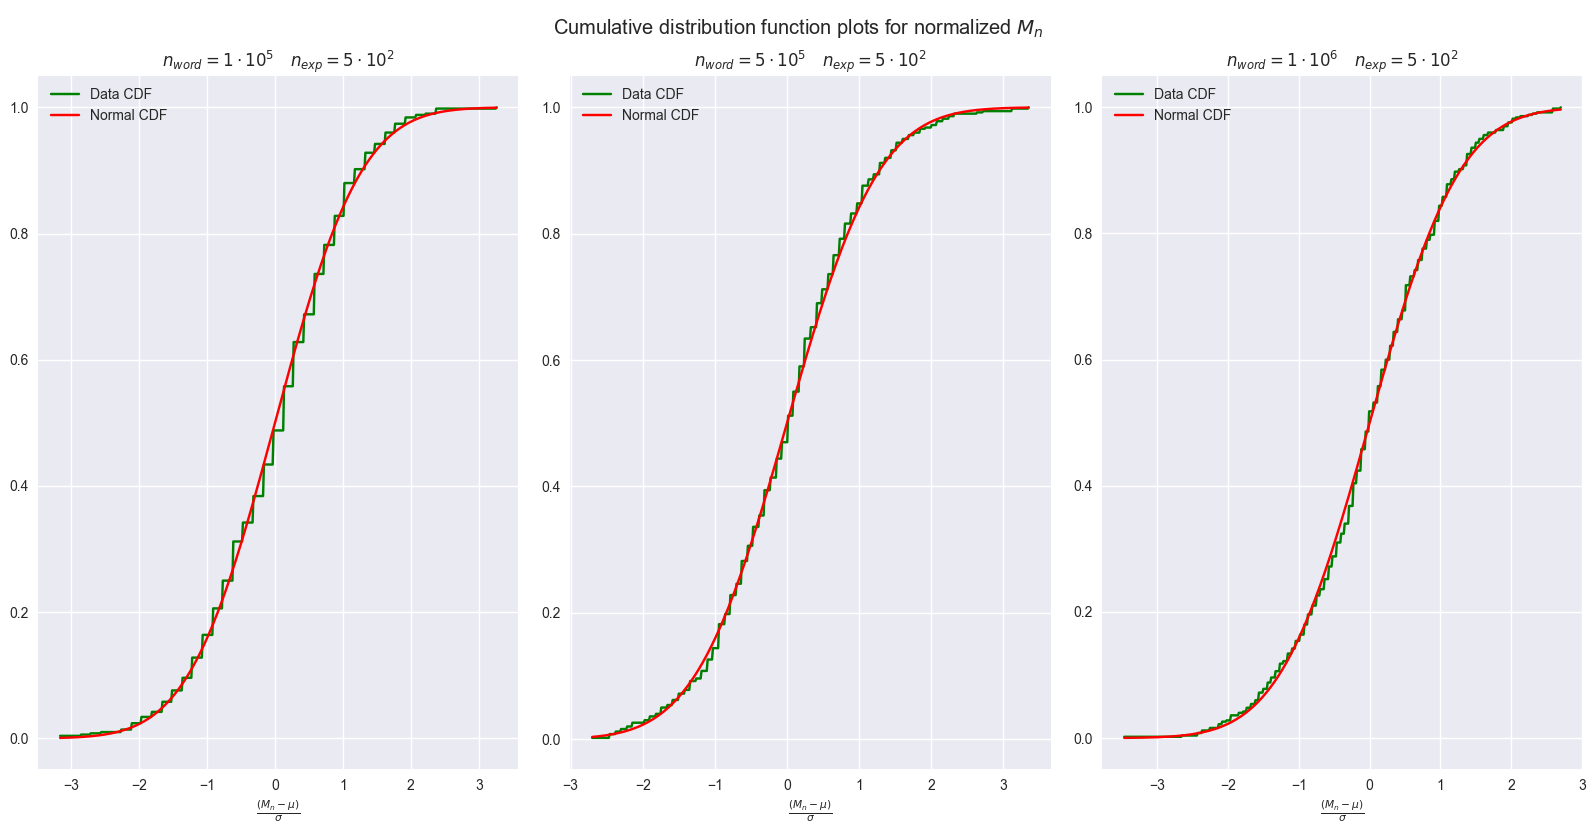
\includegraphics[width = 7cm,
        				    trim = 27cm 0 0 32,
        				    	clip=true]{cdf_1e6_500.png}
	\end{minipage} 
	}
	
	\pagebreak
	\noindent
	\centers{\question{Theoretical mean}}
	I also tried to normalize $M_n$ using theoretical expressions
	of the mean and variance. For the mean, the first order expression
	
	\centers{$E_n \sim \f{nh}{\log_2(n)}$}
	
	\noindent
	is, under $n\leq 10^6$, not sufficient to center the distribution. I conducted a numerical analysis
	of the difference between this expression and the empirical mean for growing 
	values of $n$. In particular, here is how their difference, in black, compares with
	different approximation functions 
	
	\centers{
 	 \begin{minipage}{9cm}
        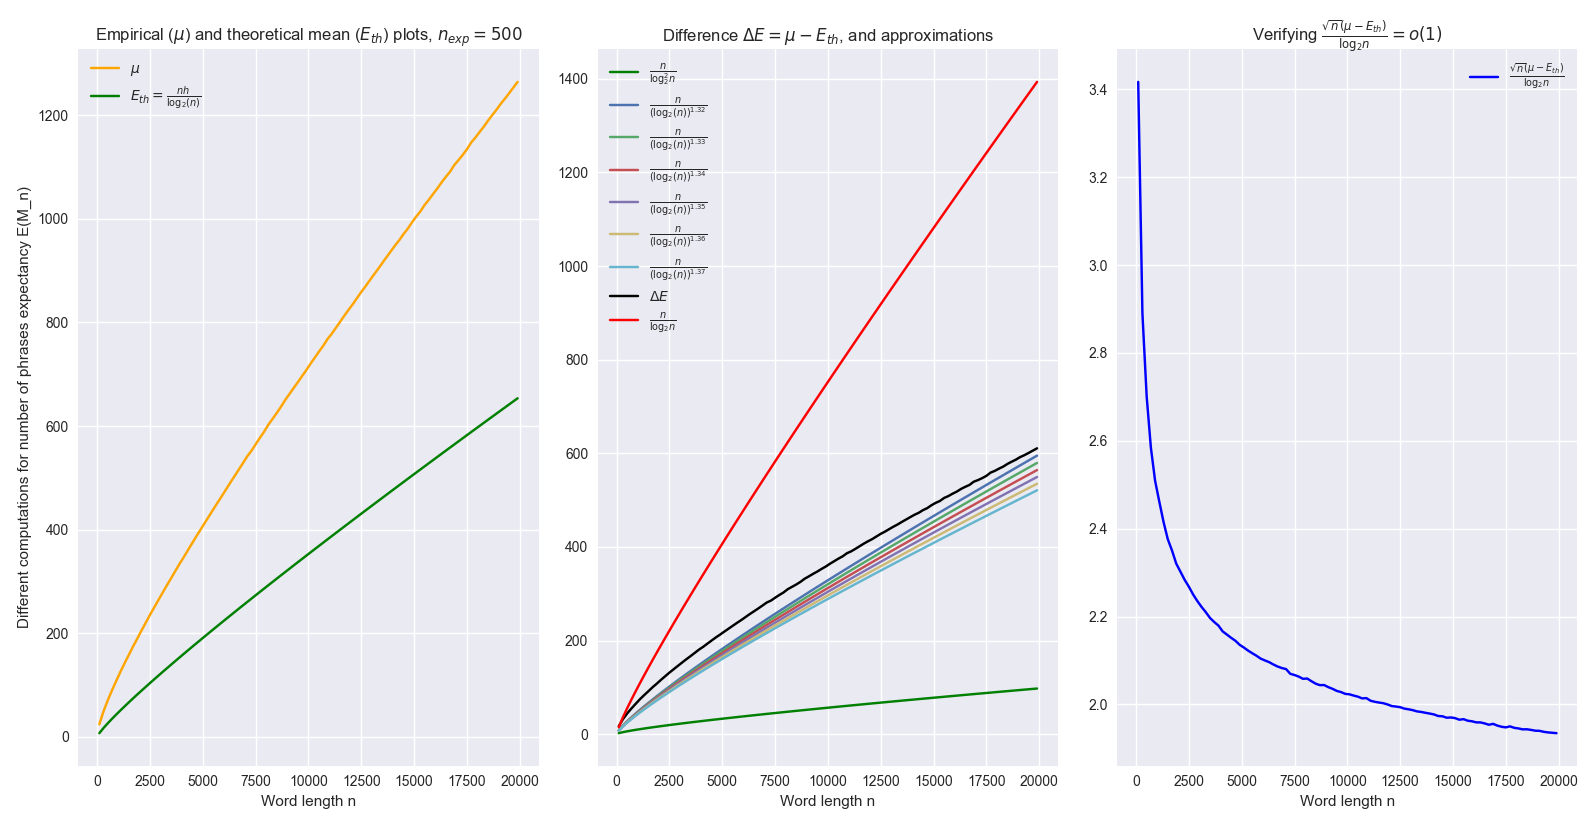
\includegraphics[width = 9cm,
        				    trim = 14cm 0 13cm 20,
        				    	clip=true]{mean_analysis_2e4_500.png}	
	\end{minipage} 
	}
	
	\noindent
	This is not troubling as it was already predicted in the formula:
	
	\centers{$E_n = 	\f{nh}{\log_2(n)} + \mathcal{O} \pa{ \f{n}{\log_2(n)} }$}
	
	\pagebreak
	\noindent
		\centers{\question{Theoretical variance}}
	For the variance, I tried to use the expression
	of $\f{H^3 \sigma^2}{n \log_2^2 (n)}$ from K. Lecket, N. Wormald and R. Neininger's paper 
		\textit{Probabilistic Analysis of Lempel-Ziv Parsing for Markov Sources} :
		
	\centers{$\sigma^2 = \sigma_0^2 + \sigma_1^2$}

	\leftcenters{where}{$\sigma_i^2 = \f{\pi_i p_{i 0} p_{i 1}}{ H^3 } \pa { \log_2 \pa{ \f{ p_{i 0} }{ p_{i 1} } }
										+ \f{H_1 - H_0}{p_{0 1} + p_{1 0}} }^2$}
	\leftcenters{with}{$\pi_0 = \f{p_{1 0}}{p_{1 0} + p_{0 1}} \qquad \pi_1 = \f{p_{0 1}}{p_{1 0} + p_{0 1}}$}
	\leftcenters{and}{$H_i = -p_{i 0} \log_2(p_{i 0}) - p_{i 1} \log_2(p_{i 1}) \qquad H = \pi_0 H_0 + \pi_1 H_1 $}
	
	\begin{remarque}
	\noindent 
	The first term in the squared part of $\sigma_i^2$ accounts for the expression of the variance for memoryless sources:
	
	\begin{egalites}
	& \ p_{i 0}\,p_{i 1} \log_2^2 \pa{ \f{p_{i 0} }{ p_{i 1} }}
		& p_{i 0} \log_2^2(p_{i 0}) + p_{i 1} \log_2^2(p_{i 1}) 
			- (- p_{i 0} \log_2(p_{i 0})  - p_{i 1} \log_2(p_{i 1}))^2 \\
		&& h_2 - h^2
	\end{egalites}
	
	\end{remarque}	
	
	\noindent
	It seems, from simulations, that this variance is too small and doesn't
	catch up with the empirical variance. Here is how they compare when plotted
	together :
	
	\centers{
 	 \begin{minipage}{11cm}
        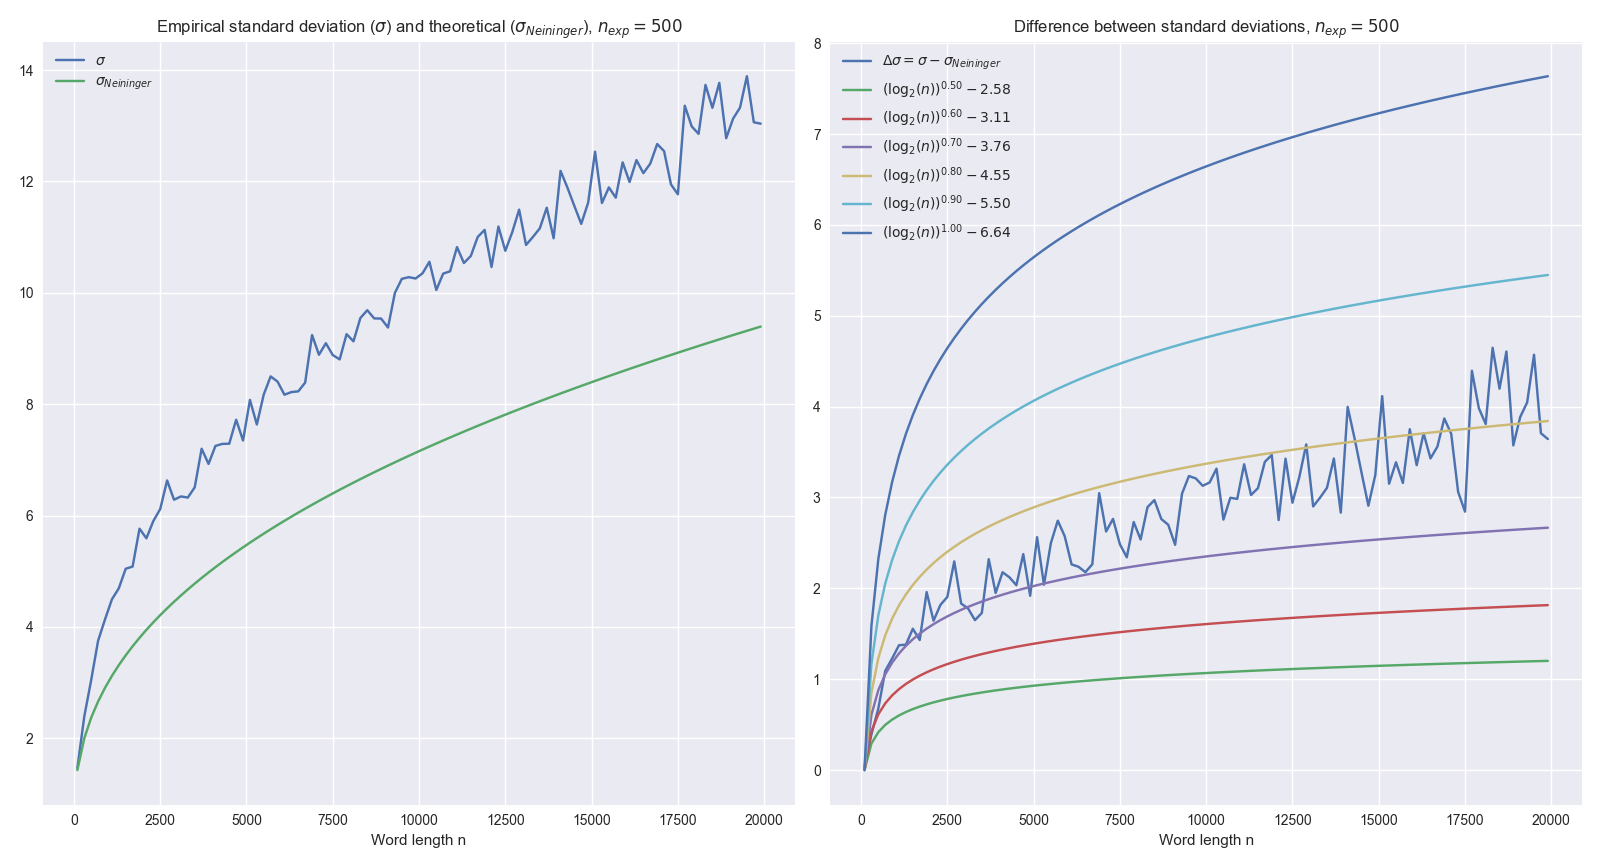
\includegraphics[width = 11cm,
        				    trim = 15 0 20cm 0,
        				    	clip=true]{std_analysis_2e4_500.png}	
	\end{minipage} 
	}
	
	\pagebreak
	\noindent
	It seems, at first glance, that the increase would asymptotically be 
	simply logarithmic
	
	\centers{
 	 \begin{minipage}{12cm}
        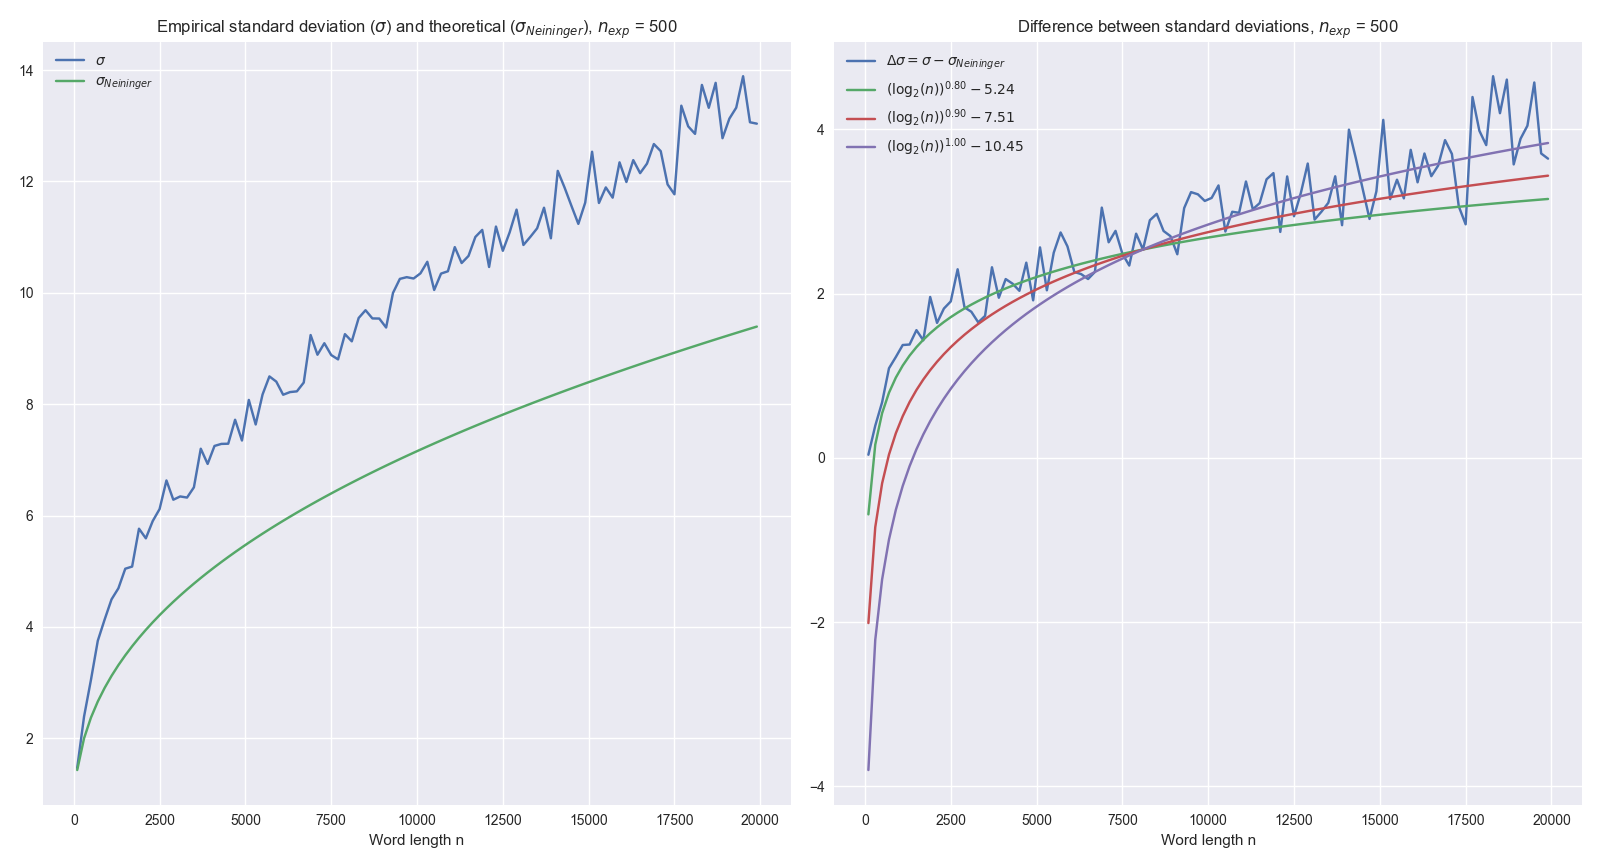
\includegraphics[width = 12cm,
        				    trim = 20.5cm 0 0 0,
        				    	clip=true]{std_analysis_approx_2e4_500.png}	
	\end{minipage} 
	}
	
	\noindent 
	
	Now, I'm trying to compute the variance using the formula from	Jacquet and Szpankowski, 
	\textit{Average profile of the Lempel-Ziv parsing scheme for a markovian source},
	using the formula for the variance $V_n$ :
	
	\centers{$h^3 V_n = -\f{\beta}{\omega} - \f2{\omega} \pi \dot{Q}^{\star} \psi - h^2$}
	\vspace{2mm}
	\begin{egalites}
	where & \omega 
			& \det \begin{matrice}
							1 & -p_{0 1} & \cdots & -p_{0 V-1} \\
							1 & -p_{1 1} & \cdots & -p_{1 V-1} \\
							\vdots & \vdots & \ddots & \vdots \\
							1 & -p_{V-1 1} & \cdots & 1 - p_{V-1 V-1} \\
						  \end{matrice}    \\[10mm]
						  
		  && (1 - p_{1 1})\, p_{0 1} & in our case \\[4mm]
	
	and & \beta 
			& \rest{\pac{\det Q''(s)}}{s=-1} \\[4mm]
			&& p_{0 0}\, p_{1 1} \ln^2 p_{0 0} \cdot \ln^2 p_{1 1}
				- p_{0 1}\, p_{1 0} \ln^2 p_{0 1} \cdot \ln^2 p_{1 0}
	\end{egalites}
	
	Finally,
	
	\begin{calculs}
		&\pi \dot{Q}^{\star} \psi
			& = &\pi_0 \, p_{1 1} \, \ln (p_{1 1}) 
					  - \pi_0\, p_{0 1} \ln (p_{0 1}) \\
			&&&		  + \pi_1 \, p_{0 0} \ln (p_{0 0})
					  - \pi_1 \, p_{1 0} \ln (p_{1 0}) \\
			&&& p_{1 1}\,\ln(p_{1 1}) + p_{0 0}\, \ln(p_{0 0}) + h 
	\end{calculs}
	
	\begin{figure}[t]
  \begin{center}
    \showthe\columnwidth % Use this to determine the width of the figure.
    \includegraphics[width=\columnwidth]{fig1.eps}
    \caption{\label{fig:sin_cos} Plot of the sine and cosine functions.}
  \end{center}
\end{figure}
					  
	
	
	
 
 
 

	 	
